
\chapter{Priprema podataka} % Main chapter title

\label{Priprema_podataka} % For referencing 





\subsection{Ontologije gena i ključne reči}



\subsection{Objedinjavanje CAFA3 i novije Svis-Prot verzije}

iz CAFA3 trening skupa izdvojeni su svi validni proteini ( dužine barem 9, i
azbukom od 20 standardnih aminokiselina). Ni u jednom trenutko ne izbacujemo
proteine manje od 40 aminokiseline jer to deo analize funkcije i nismo želeli
da ograničimo skup mogućih predikcija neuređenosti.

Informacije o Svis-Prot bazi dobijene su iz verzije 2017\_12, iz datoteke
\url{ftp://ftp.uniprot.org/pub/databases/uniprot/previous_releases/release-2017_12/knowledgebase/uniprot_sprot-only2017_12.tar.gz}.
Pomenuta verzija ima 556.196 proteina. Zbog novijeg datuma baze postoje razlike
u broju, sekvencama i  anotacijama proteina u odnosu na CAFA3 verzije proteina.

Od 66.599 validnih CAFA3 proteina 66.530 ima nepromenjen \keyword{primarni
  identifikator} \en{accession number\footnote{Pod brojem se zapravo
  podrazumeva alfanumerička oznaka.}}.  69 novih unosa(slogova\footnote{ Slog
  \en{Record} u terminima baze podataka predstavlja zapis jednog elementa u
ovom slučaju reprezentacije proteina i njegovih karakteristika.  identifkovan
je primarnim identifikatorm.  }) u Svis-Prot bazu dobijena su revizijom CAFA3
proteina koji nam nedostaju.  Ove je posledica dva moguća mehanizma:

\begin{enumerate}
  \item Unifikacija postojećih proteina u jedan novi slog. Rezultat ovog
    preslikavanja prikazan je na slici \ref{fig:unifikacija_slogova}. Analizom
    ovih promena uspešno su rekonstruisana  svega 4 nova sloga. Kako je 4
    suviše mali broj zbog jednostavnosti zanemarili smo sve slogove dobijene
    unifikacijom.

  \begin{figure}[th]
  \centering
  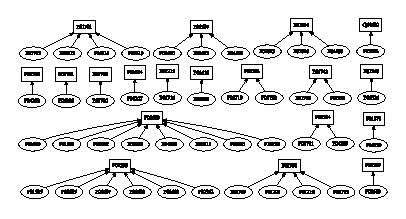
\includegraphics[scale=2]{plots/unifikacija_slogova2.eps}
  \decoRule
  \caption{Unifikacija starih(elispe) na nove slogove u Svis-Prot bazi}
  \label{fig:unifikacija_slogova}
  \end{figure}

  \item Specijalizacija jednog proteina u više različitih slogova.  Zbog moguće
    statističke redundantnosti ovi slogovi su zanemareni.
\end{enumerate}





Validini CAFA3 proteini anotirani su sa  5957 različitih GO termina Molekulske
Funkcije (MF) od kojih je 50 zamenjeno novijim terminom i izbačeno iz najnovije
\file{go.obo} datoteke. U Svis-Prot bazi nismo bili u mogućnosti da proverimo
za MF ali ukupno je zamenjeno 319 GO termina.
CAFA3 sadrži 67 MF GO termina koji se ne javljaju u Swis-Prot anotacijama.
Swis-Prot sadrži 888 MF GO termian koji se ne javljaju u CAFA3 anotacijama.
Pošto Svis-Prot treba da sadrži novije(tačnije informacije) CAFA3 anotacije
su zanemarene.

Pored anotacija Svis-Prot sadrži 194 proteina čija se sekvenca razlikuje u
odnosu na CAFA3 verziju proteina. Odlučeno je da ipak koristimo CAFA3 sekvence.


